\section{Risultati}\label{risultati}

\subsection{Tabella dei risultati}
\begin{center}
	\begin{tabular}{|c|c|c|c|c|c|}
		\hline
		\parbox{2cm}{\centering Istanza} & {Soluzione} & {Tempo(s)} & \parbox{2.75cm}{\vspace{.1cm}\centering Tempo Full Contraction(s)\vspace{.1cm}} & \parbox{2cm}{\centering Discovery time(s)} & {Errore(\%)}\\\hline
		input\_1\_6.txt & 2 & 0.00228 & 0.00007 & 0.00044 & 0.00\\\hline
		input\_2\_6.txt & 1 & 0.00174 & 0.00005 & 0.00006 & 0.00\\\hline
		input\_3\_6.txt & 3 & 0.00209 & 0.00006 & 0.00012 & 0.00\\\hline
		input\_4\_6.txt & 4 & 0.00170 & 0.00005 & 0.00009 & 0.00\\\hline
		input\_5\_10.txt & 4 & 0.01729 & 0.00015 & 0.00078 & 0.00\\\hline
		input\_6\_10.txt & 3 & 0.01288 & 0.00011 & 0.00015 & 0.00\\\hline
		input\_7\_10.txt & 2 & 0.01303 & 0.00011 & 0.00012 & 0.00\\\hline
		input\_8\_10.txt & 1 & 0.01215 & 0.00011 & 0.00013 & 0.00\\\hline
		input\_9\_25.txt & 7 & 1.34433 & 0.00134 & 0.01209 & 0.00\\\hline
		input\_10\_25.txt & 6 & 1.31912 & 0.00131 & 0.02524 & 0.00\\\hline
		input\_11\_25.txt & 8 & 1.38386 & 0.00138 & 0.00393 & 0.00\\\hline
		input\_12\_25.txt & 9 & 1.83993 & 0.00183 & 0.01214 & 0.00\\\hline
		input\_13\_50.txt & 15 & 60.01566 & 0.01666 & 0.31949 & 0.00\\\hline
		input\_14\_50.txt & 16 & 60.00023 & 0.01735 & 0.01634 & 0.00\\\hline
		input\_15\_50.txt & 14 & 60.00337 & 0.01405 & 0.01708 & 0.00\\\hline
		input\_16\_50.txt & 10 & 60.00059 & 0.01717 & 0.01396 & 0.00\\\hline
		input\_17\_75.txt & 19 & 60.04531 & 0.05812 & 0.28464 & 0.00\\\hline
		input\_18\_75.txt & 15 & 60.05066 & 0.05987 & 0.22496 & 0.00\\\hline
		input\_19\_75.txt & 18 & 60.03110 & 0.05914 & 0.16354 & 0.00\\\hline
		input\_20\_75.txt & 16 & 60.02701 & 0.05139 & 0.09496 & 0.00\\\hline
		input\_21\_100.txt & 22 & 60.00147 & 0.12987 & 2.53955 & 0.00\\\hline
		input\_22\_100.txt & 23 & 60.08396 & 0.11599 & 3.10299 & 0.00\\\hline
		input\_23\_100.txt & 19 & 60.02514 & 0.12826 & 0.12116 & 0.00\\\hline
		input\_24\_100.txt & 24 & 60.06026 & 0.12591 & 1.32756 & 0.00\\\hline
		input\_25\_125.txt & 34 & 60.20452 & 0.29368 & 1.40238 & 0.00\\\hline
		input\_26\_125.txt & 29 & 60.02135 & 0.26558 & 0.75063 & 0.00\\\hline
		input\_27\_125.txt & 36 & 60.24215 & 0.30272 & 2.94239 & 0.00\\\hline
		input\_28\_125.txt & 31 & 60.17579 & 0.26277 & 13.44911 & 0.00\\\hline
		input\_29\_150.txt & 37 & 60.16308 & 0.56227 & 1.76109 & 0.00\\\hline
		input\_30\_150.txt & 35 & 60.34957 & 0.51581 & 15.62627 & 0.00\\\hline
		input\_31\_150.txt & 41 & 60.16005 & 0.51419 & 3.07488 & 0.00\\\hline
		input\_32\_150.txt & 39 & 60.05670 & 0.53622 & 12.24101 & 0.00\\\hline
		input\_33\_175.txt & 42 & 60.22020 & 0.92646 & 11.07539 & 0.00\\\hline
		input\_34\_175.txt & 45 & 60.65118 & 0.91895 & 10.16296 & 0.00\\\hline
		input\_35\_175.txt & 53 & 60.76624 & 1.06607 & 28.81443 & 0.00\\\hline
		input\_36\_175.txt & 43 & 60.72785 & 0.84344 & 33.94806 & 0.00\\\hline
	\end{tabular}
\end{center}

\pagebreak

\begin{center}
	\begin{tabular}{|c|c|c|c|c|c|}
		\hline
		\parbox{2cm}{\centering Istanza} & {Soluzione} & {Tempo(s)} & \parbox{2.75cm}{\vspace{.1cm}\centering Tempo Full Contraction(s)\vspace{.1cm}} & \parbox{2cm}{\centering Discovery time(s)} & {Errore(\%)}\\\hline
		input\_37\_200.txt & 54 & 60.28828 & 1.58653 & 28.65111 & 0.00\\\hline
		input\_38\_200.txt & 52 & 60.42248 & 1.40517 & 2.72059 & 0.00\\\hline
		input\_39\_200.txt & 51 & 60.90992 & 1.52275 & 50.57414 & 0.00\\\hline
		input\_40\_200.txt & 61 & 60.02180 & 1.66727 & 36.01279 & 0.00\\\hline
	\end{tabular}
\end{center}

\subsection{Grafico di confronto dei tempi di esecuzione}
\begin{center}
	\begin{figure}[H]
		\centering
		\hspace{-1cm}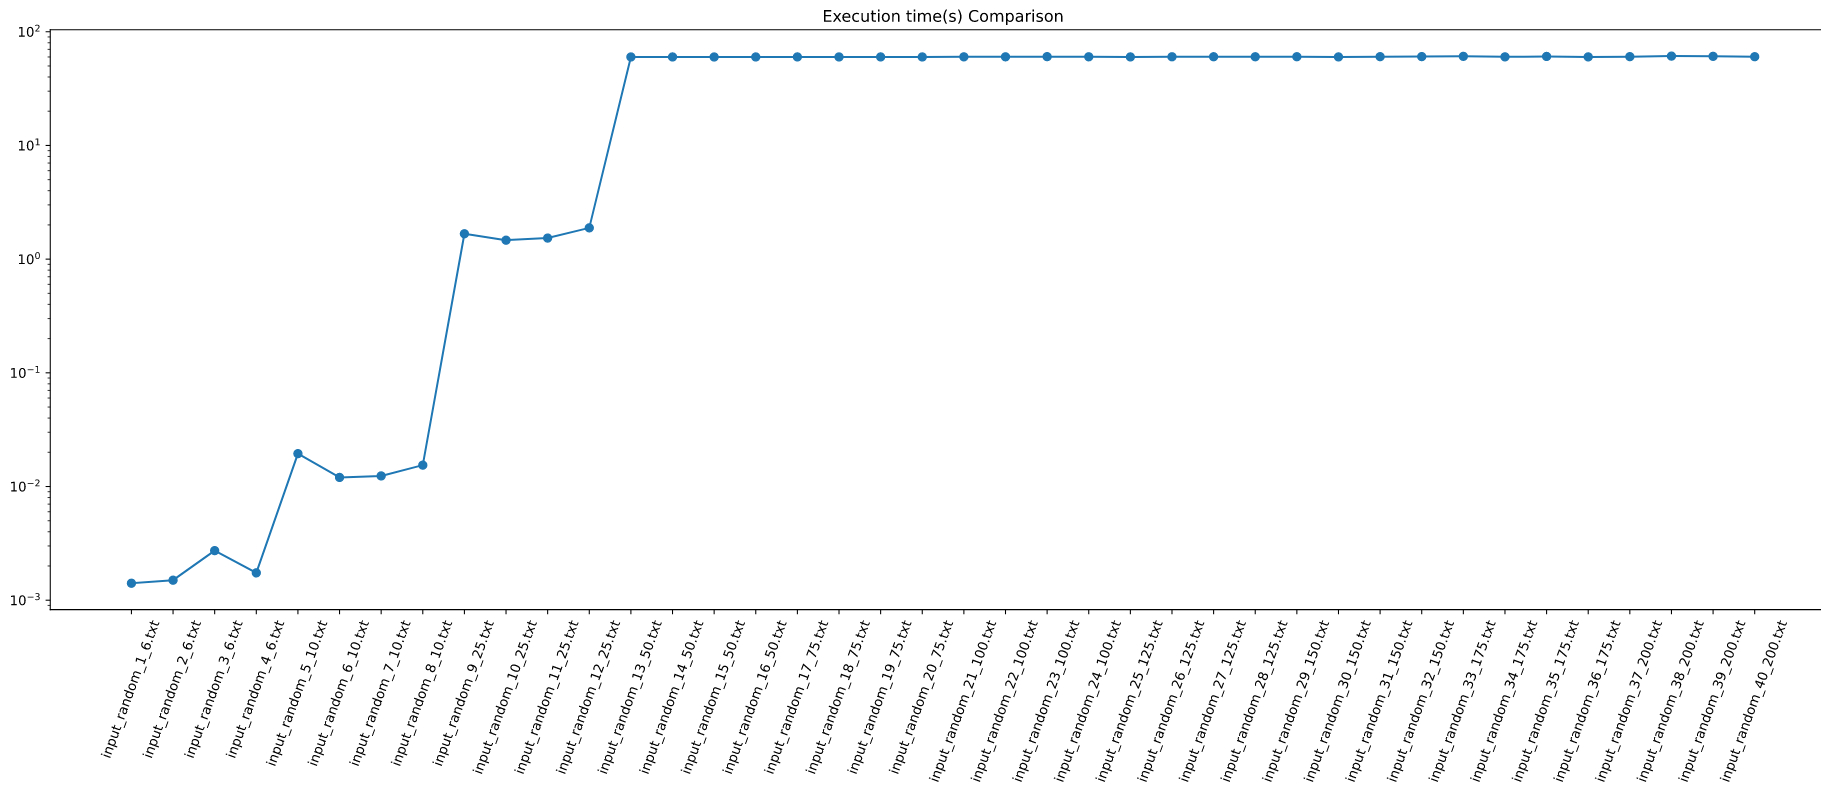
\includegraphics[width=\linewidth]{Img/exec_time_graph.jpg}
		\caption{Confronto dei tempi di esecuzione}
	\end{figure}
\end{center}

\subsection{Grafico di confronto dei tempi di Full Contraption}
\begin{center}
	\begin{figure}[H]
		\centering
		\hspace{-1cm}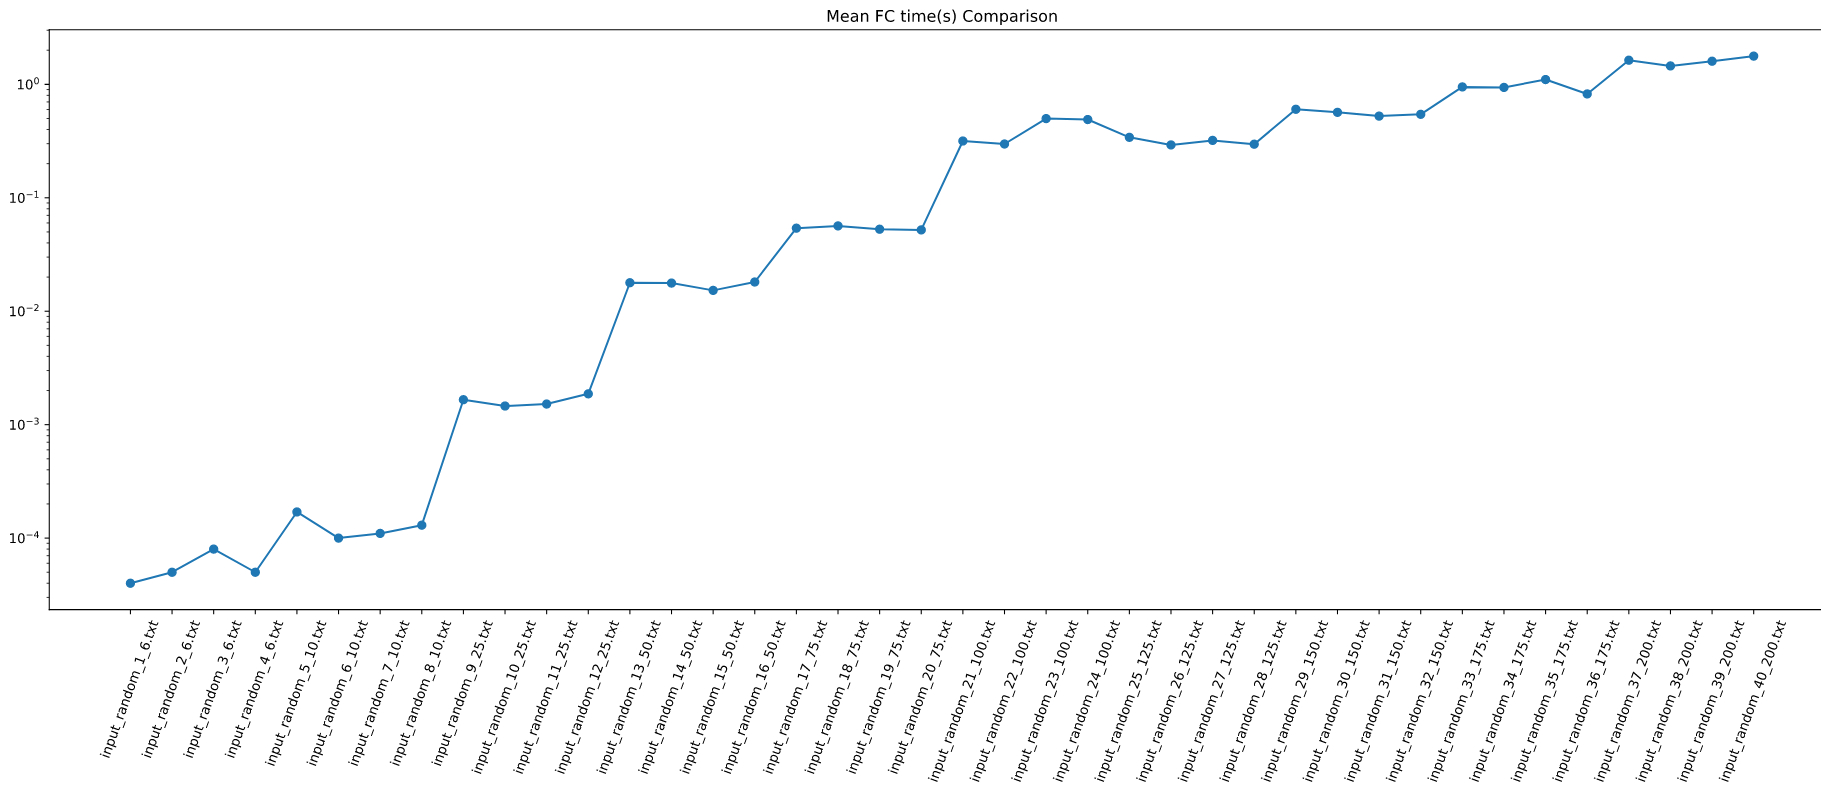
\includegraphics[width=\linewidth]{Img/fc_time_graph.jpg}
		\caption{Confronto dei tempi di Full Contraption}
	\end{figure}
\end{center}

\subsection{Grafico di confronto dei Discovery Time}
\begin{center}
	\begin{figure}[H]
		\centering
		\hspace{-1cm}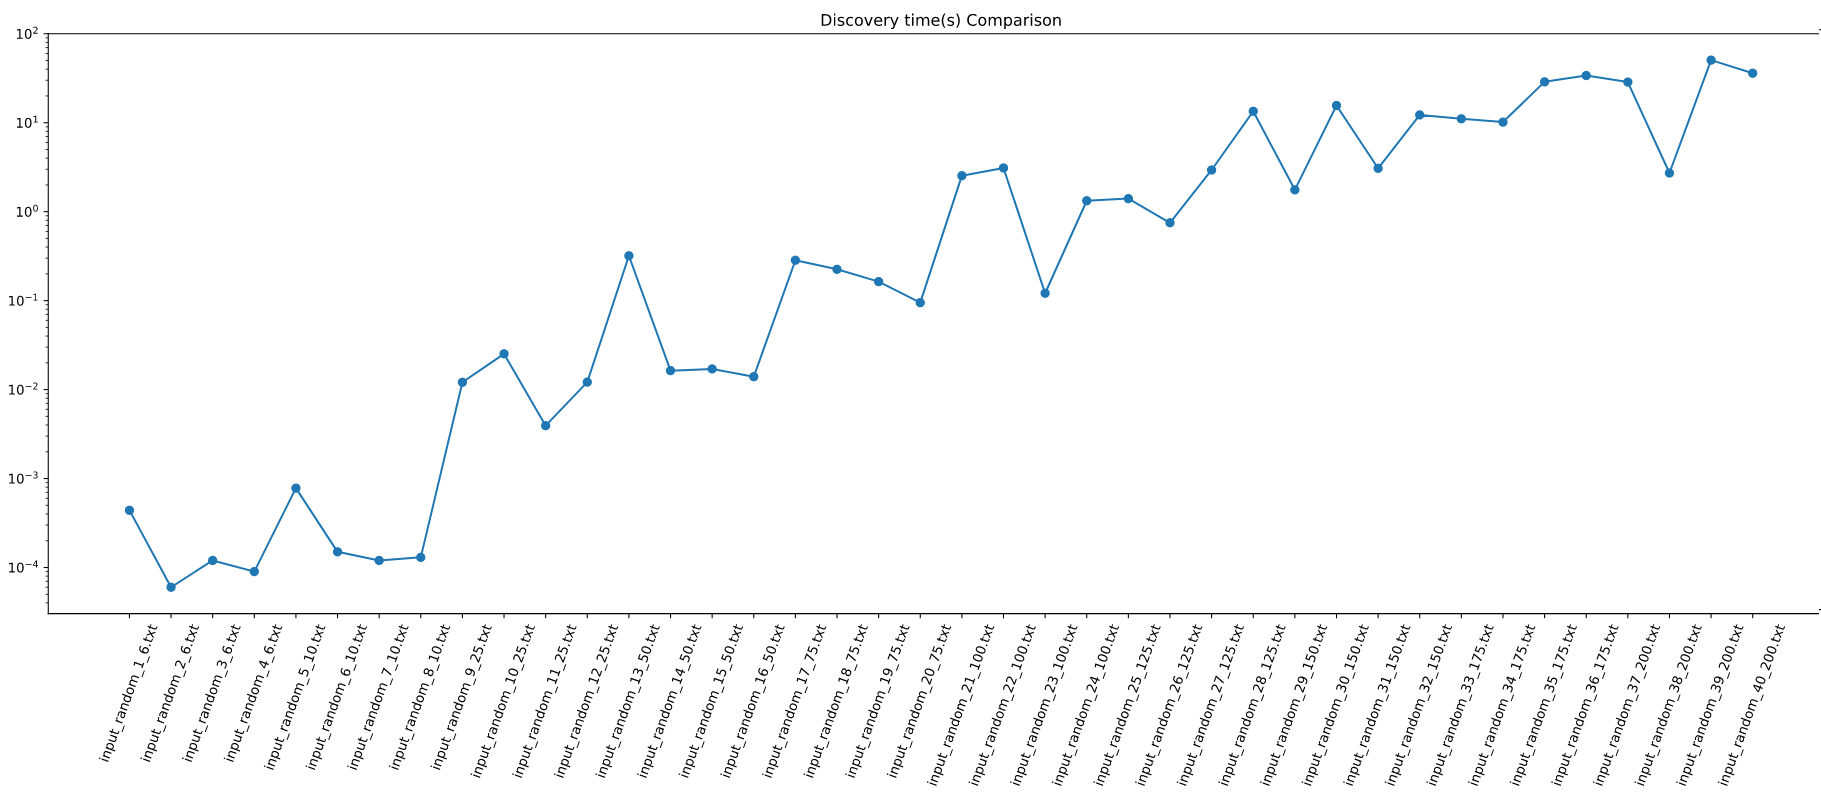
\includegraphics[width=\linewidth]{Img/disc_time_graph.jpg}
		\caption{Confronto dei Discovery Time}
	\end{figure}
\end{center}

\subsection{Grafico di confronto delle percentuali di errore}
\begin{center}
	\begin{figure}[H]
		\centering
		\hspace{-1cm}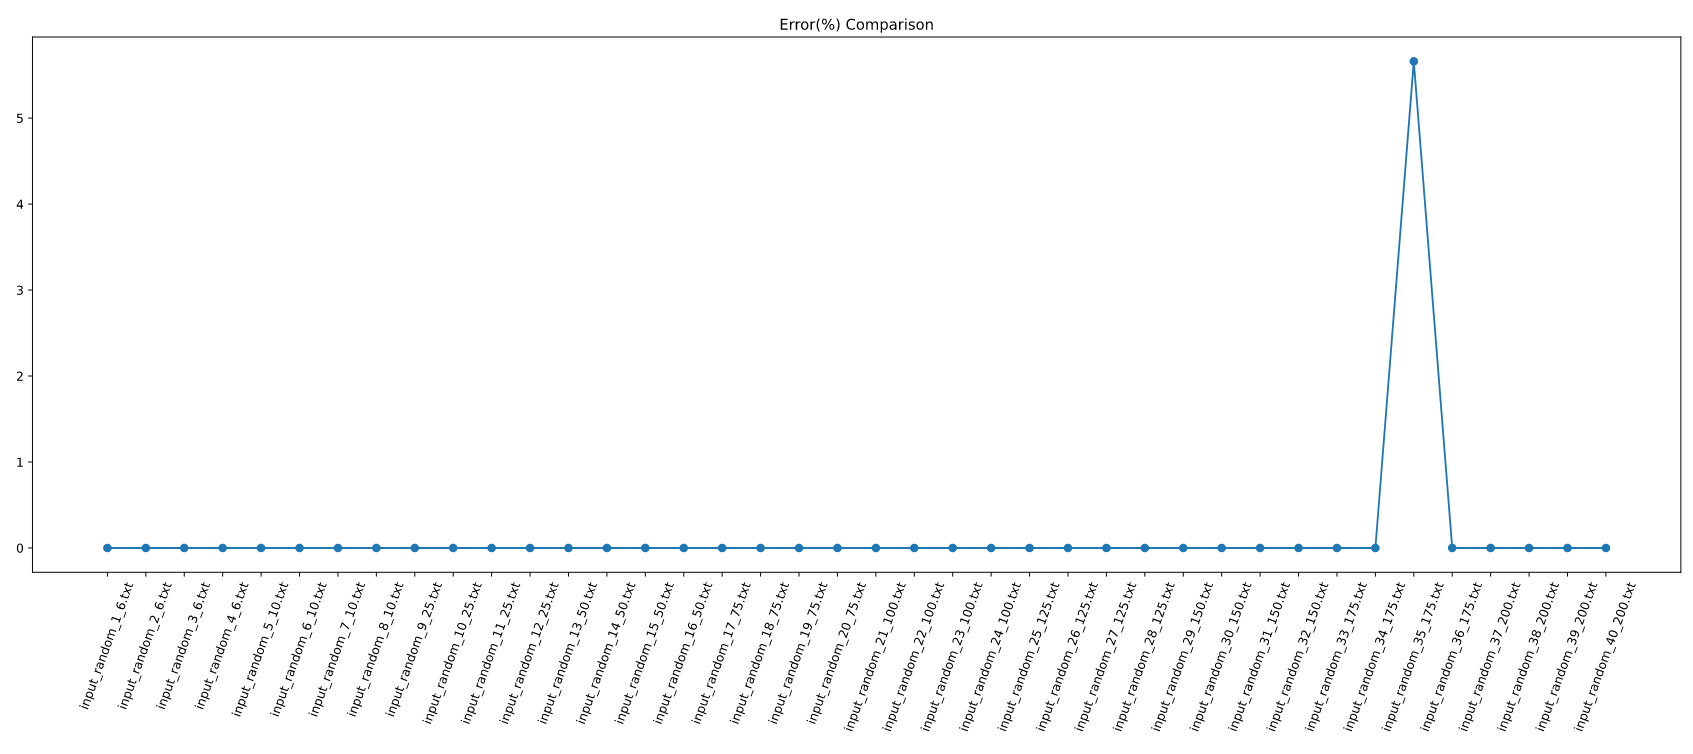
\includegraphics[width=\linewidth]{Img/err_perc_graph.jpg}
		\caption{Confronto delle percentuali di errore}
	\end{figure}
\end{center}

\pagebreak